% The Silent Tax: How Typos Reshape Reasoning in Thinking LLMs
% NLP Course 2025/2026, Tel Aviv University.
%
% Built against the official ACL Overleaf template. Drop acl.sty, acl_natbib.bst
% and the ACL .cls-adjacent files next to this file (see README.md). If they are
% absent the document still compiles with a plain fallback preamble.

\documentclass[11pt]{article}

\IfFileExists{acl.sty}{%
  \usepackage[final]{acl}%
}{%
  % Fallback so the document still builds without the ACL style files.
  \usepackage[margin=1in]{geometry}%
  \usepackage{natbib}%
  \providecommand{\And}{\quad}%
  \providecommand{\AND}{\quad}%
  \bibliographystyle{plainnat}%
}

\usepackage{times}
\usepackage{latexsym}
\usepackage[T1]{fontenc}
\usepackage[utf8]{inputenc}
\usepackage{microtype}
\usepackage{graphicx}
\usepackage{booktabs}
\usepackage{amsmath}
\usepackage{amssymb}
\usepackage{multirow}
\usepackage{xcolor}

\graphicspath{{figures/}}

\newcommand{\typo}[1]{\textcolor{red!75!black}{\textbf{#1}}}
\newcommand{\pp}{\,pp}

\title{The Silent Tax: How Typos Reshape Reasoning in Thinking LLMs}

\author{%
  Shiran Hamami \\ 207487026 \\ \small\texttt{shiranhamami@mail.tau.ac.il}
  \And
  Dolev Abudi \\ 323096099 \\ \small\texttt{dolevabudi@mail.tau.ac.il}
  \AND
  Ron Shtricker \\ 209524552 \\ \small\texttt{ronshtricker@mail.tau.ac.il}
  \And
  Ido Azoulay \\ 212710958 \\ \small\texttt{idoazoulay1@mail.tau.ac.il}
}

\begin{document}
\maketitle

\begin{abstract}
Reasoning-distilled language models are increasingly trusted for math and
science, yet the questions real users type contain typos. We build a controlled
typo generator that independently varies \emph{how many} words are corrupted
(25/50/75\% of eligible words) and \emph{what fraction} of the corruptions land
on other valid English words (10/40/70\%), and we apply it to 500 questions each
from GSM8K, MATH-500 and ARC-Challenge. Running
DeepSeek-R1-Distill-Qwen-7B over the resulting $3\times10$ grid (15{,}000
traces, plus 15{,}000 more for controls and mitigations) we find a large,
monotone accuracy tax: GSM8K falls from 91.4\% to 60.4\% ($-31.0\pp$;
$164/480$ paired right-to-wrong flips, $p<10^{-6}$), with smaller but
significant losses on ARC ($-10.4\pp$) and MATH-500 ($-8.2\pp$). Holding the
number of typos fixed, shifting them onto real words costs a further
$14.1\pp$ on GSM8K ($p=1.3\times10^{-7}$); per typo, a real-word corruption is
$1.9\times$ (GSM8K) to $5.1\times$ (ARC) more damaging than a non-word one. Our
central hypothesis --- that real-word typos cause \emph{silent} failures ---
is refuted: an LLM judge shows the model notices real-word corruptions
\emph{more} often, not less, and the dominant failure mode is
noticed-but-unrecoverable (58--59\% accuracy when the model flags a typo it
cannot fix, versus 84\% when it reads through silently). The lexical
signature of typo stress is \emph{hedging} (``maybe'' $+5.7$/1k tokens) while
classical self-correction markers (``wait, actually'', ``double-check'')
stay flat or decline. Finally, every lightweight mitigation fails: warning the
model is null ($-0.5\pp$), asking it to rewrite the question first actively
hurts ($-4.7\pp$), and an external spell checker restores 55\% of typos when
10\% are real words but only 25\% when 70\% are.
\end{abstract}

%-------------------------------------------------------------------------------
\section{Introduction}
\label{sec:intro}

Chain-of-thought prompting and, more recently, reasoning-distilled models have
sharply raised the accuracy ceiling on mathematical and scientific
benchmarks \citep{wei2022,deepseekr1}. Benchmark inputs, however, are
copy-edited prose. The questions people actually type are not: they contain
transposed letters, dropped characters and adjacent-key slips. A model that is
excellent on clean GSM8K but brittle on the same question with three typos is
less useful than its benchmark score suggests and --- because the failure is
invisible to the user --- more dangerous.

Prior work establishes that typos hurt standard LLMs and attributes much of the
damage to subword tokenization \citep{gan2024,chai2024,zhao2025}, but it reports
final accuracy only, on models that do not emit a long deliberate reasoning
trace. Reasoning models are exactly where the question becomes interesting: they
have thousands of tokens in which they could, in principle, notice a corruption,
repair it, and recover. Do they?

\begin{figure}[t]
\centering
\small
\setlength{\fboxsep}{5pt}
\fbox{\begin{minipage}{0.93\columnwidth}
\textbf{Clean (model answers 18, correct)}\\[2pt]
{\footnotesize Janet's ducks lay 16 eggs per day. She eats three for
breakfast every morning and bakes muffins for her friends every day with four.
She sells the remainder at the farmers' market daily for \$2 per fresh duck egg.
How much in dollars does she make every day at the farmers' market?}\\[6pt]
\textbf{25\% typos, 40\% of them real words (model answers 26, wrong)}\\[2pt]
{\footnotesize Janet's \typo{duck} lay 16 eggs per \typo{adqy}. \typo{Sje}
\typo{east} \typo{rthere} for breakfast every morning and bakes muffins for
\typo{uher} \typo{friend} every \typo{azy} with four. She sells the remainder at
the farmers' market daily for \$2 per \typo{resh} duck egg. How much in dollars
does she make every day at the \typo{faremrs}' market?}\\[6pt]
{\scriptsize\ttfamily
eats\,$\to$\,east\quad ducks\,$\to$\,duck\quad three\,$\to$\,rthere\\
friends\,$\to$\,friend\quad fresh\,$\to$\,resh\quad her\,$\to$\,uher}
\end{minipage}}
\caption{A single GSM8K item under our generator. Numbers and \LaTeX{} are
protected; only alphabetic words are corrupted. The two \emph{real-word} typos
(\texttt{eats}\,$\to$\,\texttt{east},
\texttt{ducks}\,$\to$\,\texttt{duck}) are invisible to a spell checker. The
model loses the ``three eaten'' quantity and answers 26 instead of 18.}
\label{fig:teaser}
\end{figure}

We answer this with a controlled two-axis design. Our generator decouples the
\emph{amount} of corruption (typo rate) from its \emph{kind} (the share of
typos that produce another valid English word), so that a real-word effect can
be measured at a fixed number of typos on the very same questions --- a
comparison prior work does not make. We run
DeepSeek-R1-Distill-Qwen-7B \citep{deepseekr1} over the full grid on three
datasets with different reasoning profiles, and instrument the reasoning trace
itself with a word-level alignment analysis and an LLM judge.

Our contributions are: (i) a controlled rate\,$\times$\,real-word grid ($3$
datasets $\times$ $10$ configurations $\times$ $500$ questions) in which every
condition contains the same questions, enabling paired McNemar tests rather than
accuracy differences alone (\S\ref{sec:method}); (ii) evidence that the typo tax
is large, monotone and dataset-dependent, and that it is a
\emph{reasoning-quality} loss rather than a truncation artifact
(\S\ref{sec:accuracy}); (iii) a per-typo logistic analysis and a controlled
paired test showing real-word typos are substantially more damaging than
non-word typos (\S\ref{sec:realword}); (iv) a refutation of our own
pre-registered ``silent failure'' hypothesis --- the harm comes from
\emph{noticed-but-unrepairable} corruption, not unnoticed corruption
(\S\ref{sec:repair}); and (v) negative results for all three lightweight
mitigations, with a mechanistic explanation for why spell checking cannot help
(\S\ref{sec:mitigations}).

%-------------------------------------------------------------------------------
\section{Background and Related Work}
\label{sec:related}

\paragraph{Character-level brittleness.}
\citet{belinkov2018} show that both synthetic and natural character noise breaks
neural machine translation and that robustness to one noise type does not
transfer to another. Adversarial NLP work weaponises this: HotFlip
\citep{ebrahimi2018} finds minimal character flips that reverse a classifier,
TextFooler \citep{jin2020} does the same at the word level, and PromptBench
\citep{zhu2024} shows character-level perturbations remain among the most
effective attacks on instruction-tuned LLMs. \citet{pruthi2019} propose a robust
word-recognition front-end as a defence --- the ancestor of the spell-checker
mitigation we test in \S\ref{sec:mitigations}.

\paragraph{Typos and modern LLMs.}
Closest to us, \citet{gan2024} inject adversarial typos into math questions and
report accuracy drops for instruction-tuned LLMs; \citet{chai2024} attribute
much of the damage to subword tokenization, showing that a misspelled word
fragments into sub-tokens whose embeddings carry little of the original meaning;
and \citet{zhao2025} extend the evaluation multilingually. All three measure
final accuracy on non-reasoning models. Two gaps remain. First, none separates
corruption \emph{amount} from corruption \emph{kind}: a typo that yields a
non-word (\texttt{triangle}\,$\to$\,\texttt{trianlge}) and one that yields a
different real word (\texttt{sum}\,$\to$\,\texttt{sun}) attack the model through
different channels --- the first fragments the tokenizer, the second is
tokenized perfectly and silently changes the meaning --- yet they are pooled.
Second, none inspects the reasoning trace.

\paragraph{Reasoning traces and self-correction.}
Reasoning-distilled models such as DeepSeek-R1 \citep{deepseekr1} externalise a
long deliberation before answering, making their intermediate behaviour
observable. Whether that deliberation faithfully reflects the computation is
contested \citep{turpin2023}, and \citet{huang2024} show that LLMs generally
cannot self-correct reasoning errors without external feedback. Our setting is a
sharp test case: the error is not in the model's reasoning but in its input, is
in principle detectable from the text alone, and the model has thousands of
tokens in which to detect it.

%-------------------------------------------------------------------------------
\section{Method}
\label{sec:method}

\subsection{Controlled typo generation}
\label{sec:generator}

Given a question, we tokenise it into words and mark a word \emph{eligible} if
it is alphabetic, at least two characters long, and not in a 15-word function
list (\texttt{a, an, and, as, at, by, for, if, in, is, of, on, or, the, to}).
Numbers, currency, \LaTeX{} math and \LaTeX{} commands are placed in
\emph{protected spans} and never touched, so every configuration of a question
is arithmetically identical to the clean one.

We then sample $n=\max(1,\lceil r\cdot|E|\rfloor)$ eligible words, where $r$ is
the \textbf{typo rate} and $E$ the eligible set, and corrupt each with one of
four keyboard-plausible techniques, sampled with weights chosen so that the mix
resembles observed human typing rather than a uniform prior:
adjacent-key replacement using a QWERTY adjacency map (0.40,
\texttt{math}\,$\to$\,\texttt{nath}), character deletion (0.20,
\texttt{triangle}\,$\to$\,\texttt{triagle}), character insertion (0.20,
\texttt{solve}\,$\to$\,\texttt{solvve}) and transposition (0.20,
\texttt{form}\,$\to$\,\texttt{fomr}). With probability $0.10$ a second edit is
applied to the same word.

The second axis is the \textbf{real-word ratio} $\rho$: the fraction of the $n$
corrupted words that must land on another word in the NLTK English lexicon. For
each selected word we enumerate the full distribution of single-edit candidates,
partition it into real-word and non-word outcomes, and sample so that the
realised count matches $\lfloor \rho n\rfloor$ plus a Bernoulli draw for the
fractional part. Non-word draws retry up to 10 times, and any accidental real
word that survives is counted honestly. This is the mechanism that lets us hold
$n$ fixed and vary only the \emph{kind} of corruption.

We use $r\in\{25,50,75\}\%$ and $\rho\in\{10,40,70\}\%$, giving nine typo
configurations plus \texttt{clean}. The sampler is seeded identically across
configurations, so question $i$ is the same question in all ten conditions and
every comparison is paired.

\subsection{Datasets and statistics}
\label{sec:data}

We use 500 questions from each of three benchmarks chosen to span reasoning
regimes: \textbf{GSM8K} test \citep{cobbe2021}, arithmetic word problems where
the text carries the entire problem structure; \textbf{MATH-500}
\citep{hendrycks2021,lightman2024}, competition problems where much of the
content is protected \LaTeX{}; and \textbf{ARC-Challenge} \citep{clark2018},
four-way multiple-choice science questions where an answer can be recovered from
partial understanding. Table~\ref{tab:datastats} reports the resulting
corruption statistics.

\begin{table}[t]
\centering\small
\begin{tabular}{lrrrr}
\toprule
 & GSM8K & MATH-500 & ARC-C \\
\midrule
questions            & 500  & 500  & 500 \\
mean words           & 45.8 & 31.5 & 23.5 \\
median words         & 43   & 26   & 20 \\
\midrule
typos @ $r{=}25$     & 7.6  & 4.0  & 4.2 \\
typos @ $r{=}50$     & 15.3 & 7.9  & 8.3 \\
typos @ $r{=}75$     & 22.9 & 11.8 & 12.4 \\
\midrule
real ratio @ $\rho{=}10$ & 0.099 & 0.096 & 0.106 \\
real ratio @ $\rho{=}40$ & 0.397 & 0.386 & 0.386 \\
real ratio @ $\rho{=}70$ & 0.693 & 0.637 & 0.642 \\
\midrule
total typos          & 68{,}739 & 35{,}685 & 37{,}248 \\
\bottomrule
\end{tabular}
\caption{Dataset and corruption statistics. Realised real-word ratios track the
targets closely; the shortfall at $\rho{=}70$ on MATH-500 and ARC reflects short
words with few real-word neighbours. Across all datasets the realised technique
mix is 36--37\% replace, 32\% delete, 16\% insert, 15\% transpose, with
10.0--10.2\% two-edit words.}
\label{tab:datastats}
\end{table}

Note that MATH-500 receives far fewer typos per question than GSM8K at the same
rate ($11.8$ vs.\ $22.9$ at $r{=}75$) precisely because so much of a competition
problem is protected mathematics. This is a genuine property of the domain, not
a confound we could remove, and it is one reason MATH-500 degrades least.
%-------------------------------------------------------------------------------
\section{Experimental Setup}
\label{sec:setup}

\paragraph{Models.}
Our subject model is \texttt{DeepSeek-R1-Distill-Qwen-7B}
\citep{deepseekr1}, served through an OpenAI-compatible router endpoint. We
decode with temperature $0.6$ and top-$p$ $0.95$ (the model card defaults), one
sample per question. Generation caps are 20{,}000 new tokens for GSM8K and
17{,}000 for MATH-500 and ARC. As a \textbf{non-reasoning control} we run
\texttt{Qwen2.5-7B-Instruct} \citep{qwen25} --- the same family and parameter
count, without reasoning distillation --- over the identical grid on MATH-500
and ARC. Our \textbf{judge} is \texttt{Llama-3.3-70B-Instruct}
\citep{llama3} at temperature $0$.

\paragraph{Prompts.}
Math items are prompted with the question followed by \emph{``Please reason step
by step, and put your final answer within \texttt{\textbackslash boxed\{\}}.''}
Multiple-choice items list the four options with shuffled labels and ask for the
boxed letter. Typos are injected only into the question text; the instruction
suffix is always clean.

\paragraph{Scoring.}
We use a deliberately strict extraction policy. The answer is read
\emph{only} from the text after the closing \texttt{</think>} tag, so a
lucky-looking number inside the deliberation cannot be credited. A trace that
hits the token cap without emitting an answer is scored \texttt{unanswered}
rather than wrong. GSM8K is graded by normalised numeric match, MATH-500 by
symbolic equivalence (\texttt{math\_verify}, so $1/2 \equiv 0.5 \equiv
\frac{1}{2}$), and ARC by exact letter match. We report
\emph{answered-only accuracy} $\mathrm{acc}_a$ (correct $/$ answered) as the
headline number, and give $n_{\text{answered}}$ alongside it so that the
truncation channel is always visible; \S\ref{sec:accuracy} decomposes the two.

\paragraph{Statistics.}
Because every condition contains the same 500 questions, we test the paired
quantity directly: we report right-to-wrong and wrong-to-right \textbf{flip}
counts with a continuity-corrected \textbf{McNemar} test on questions answered
in both conditions, and bootstrap 95\% CIs (10k resamples) on accuracies. An
unpaired accuracy difference conflates the typo effect with per-question
difficulty; the flip asymmetry does not.

\paragraph{Trace instrumentation.}
We measure trace behaviour two ways. (i) \emph{Word-level alignment}: for every
corrupted word we search the trace for the original word, the corrupted form, or
an explicit correction, classifying each typo as \emph{silently fixed},
\emph{flagged}, \emph{misread} or \emph{not used}. (ii) \emph{LLM judge}
\citep{zheng2023}: the judge sees the clean question, the typo question, the
corrupted word pairs and
the trace, and returns a 0--4 self-doubt rating plus one repair label from
\{\textsc{silent\_readthrough}, \textsc{explicit\_notice\_fix},
\textsc{explicit\_notice\_nofix}, \textsc{misread\_wrong\_word},
\textsc{derailed}, \textsc{unclear}, \textsc{not\_applicable}\}, with a verbatim
quote as evidence. We validate it two ways: 85.7\% of its quotes are verbatim
substrings of the trace, and on \texttt{clean} traces it returns
\textsc{not\_applicable} 99.4\% of the time --- a sanity check it could easily
have failed.

%-------------------------------------------------------------------------------
\section{Results}
\label{sec:results}

\begin{figure*}[t]
\centering
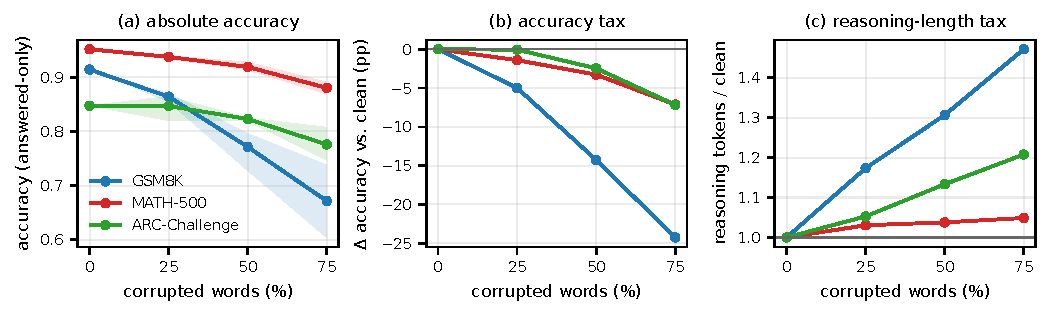
\includegraphics[width=0.94\textwidth]{fig1_accuracy.pdf}
\caption{The typo tax. \textbf{Left}: answered-only accuracy across the
rate\,$\times$\,real-word grid. \textbf{Centre}: change from \texttt{clean} in
percentage points. \textbf{Right}: reasoning length relative to \texttt{clean}.
Degradation is monotone in typo rate on all three datasets and steepest on
GSM8K, where the text carries the whole problem. Reasoning gets
\emph{longer} under typos on every dataset, so the accuracy loss is not the
model giving up early.}
\label{fig:accuracy}
\end{figure*}

\subsection{Typos impose a large, monotone accuracy tax}
\label{sec:accuracy}

Figure~\ref{fig:accuracy} and Table~\ref{tab:fullacc} (appendix) give the full
grid. On GSM8K, answered-only accuracy falls from $91.4\%$ (95\% CI
$[88.8, 93.8]$) on clean text to $60.4\%$ $[53.6, 62.4]$ at the hardest setting
($r{=}75$, $\rho{=}70$) --- a $31.0\pp$ loss from perturbations that leave every
number and every question intact. ARC falls $10.4\pp$ ($85.0\to74.7$) and
MATH-500 $8.2\pp$ ($95.2\to86.9$). Degradation is monotone in the typo rate on
all three datasets.

The paired flip analysis (Table~\ref{tab:fullflips}, appendix) makes the effect
unambiguous. At $r{=}75,\rho{=}70$ GSM8K shows $164$ right-to-wrong against only
$14$ wrong-to-right flips out of $480$ jointly answered questions (net
$31.3\pp$, McNemar $p<10^{-6}$); ARC shows $73$ vs.\ $23$ (net $11.3\pp$,
$p=5.7\times10^{-7}$) and MATH-500 $46$ vs.\ $7$ (net $7.9\pp$,
$p=1.8\times10^{-7}$). GSM8K is significantly hurt from the mildest
configuration onward ($p=6.2\times10^{-4}$ at $r{=}25,\rho{=}10$), whereas
MATH-500 and ARC are indistinguishable from clean until $r{=}50$ and $r{=}75$
respectively. The tax therefore scales with how much of the problem lives in
prose: severe for arithmetic word problems, moderate for multiple-choice science
where the options provide redundancy, and mild for competition math where the
load-bearing content is protected \LaTeX{}.

\paragraph{This is a quality loss, not a truncation artifact.}
One might worry that typos simply make traces run past the token cap. They do
not. Reasoning gets \emph{longer} under typos on every dataset --- GSM8K rises
from 1{,}582 to 2{,}594 mean generated tokens ($+64\%$ at $r{=}75,\rho{=}40$),
MATH-500 from 2{,}927 to 3{,}138, ARC from 1{,}154 to 1{,}453 --- while answered
counts stay high (Table~\ref{tab:fullacc}). Decomposing the GSM8K
strict-accuracy drop at $r{=}75,\rho{=}70$ into a completion component and a
quality component gives $-0.024$ versus $-0.310$: $93\%$ of the damage is
quality. The model does not give up; it thinks longer and still gets it wrong.
Consistently, on clean GSM8K a wrong answer is preceded by $2.46\times$ as many
tokens as a correct one, and the ratio persists under typos ($2.00\times$):
long deliberation marks trouble, not recovery.

\subsection{Real-word typos are the expensive ones}
\label{sec:realword}

\begin{figure*}[t]
\centering
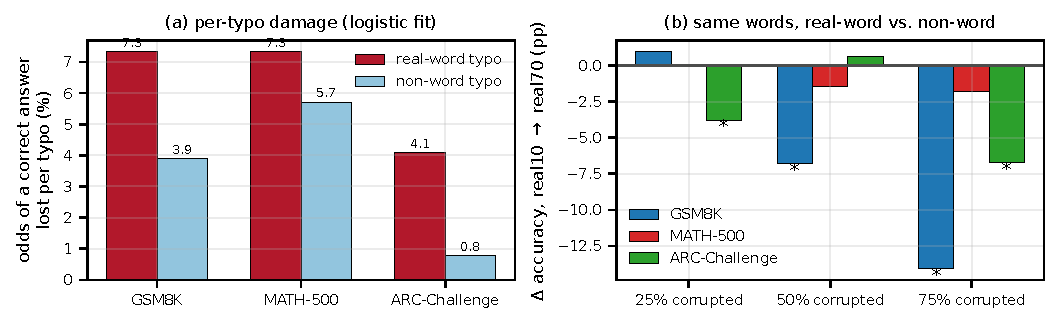
\includegraphics[width=0.9\textwidth]{fig2_realword.pdf}
\caption{The real-word effect. \textbf{Left}: multiplicative loss in the odds of
a correct answer per additional typo, from a logistic regression with separate
real-word and non-word counts. \textbf{Right}: controlled paired comparison ---
same questions, same number of typos, only the real-word share changes;
$^{*}$ marks McNemar $p<0.05$.}
\label{fig:realword}
\end{figure*}

Because our two axes are independent, we can ask what a typo costs
\emph{conditional on how many there are}. We fit, per dataset, a logistic
regression of correctness on the number of real-word and non-word typos in the
question. The per-typo odds multipliers are: GSM8K $0.927$ (real) vs.\ $0.961$
(non-word), MATH-500 $0.927$ vs.\ $0.943$, ARC $0.959$ vs.\ $0.992$. Converting
to loss per typo, a real-word corruption is $1.9\times$ more damaging than a
non-word one on GSM8K, $1.3\times$ on MATH-500, and $5.1\times$ on ARC.

The controlled paired test confirms it. Fixing $r{=}75$ on GSM8K and moving only
the real-word share from $10\%$ to $70\%$ --- identical questions, identical
typo counts --- costs $14.1\pp$ ($109$ right-to-wrong vs.\ $43$ wrong-to-right,
$n{=}468$, $p=1.3\times10^{-7}$), and the effect is graded
($10\to40$: $-5.8\pp$, $p=0.024$; $40\to70$: $-7.8\pp$, $p=0.003$). At $r{=}50$
it is $-6.8\pp$ ($p=0.002$); at $r{=}25$ it is null, i.e.\ a handful of typos of
either kind is survivable and the real-word channel only bites once the text is
substantially degraded. On ARC the same test gives $-6.7\pp$ at $r{=}75$
($p=9.5\times10^{-4}$); on MATH-500 it is not significant at any rate, which is
consistent with its much smaller per-question typo budget. This inverts the
tokenization story: the corruptions that survive tokenization intact are the
ones that do the most damage per unit.

\subsection{Repair behaviour: noticed, but not repaired}
\label{sec:repair}

\begin{figure*}[t]
\centering
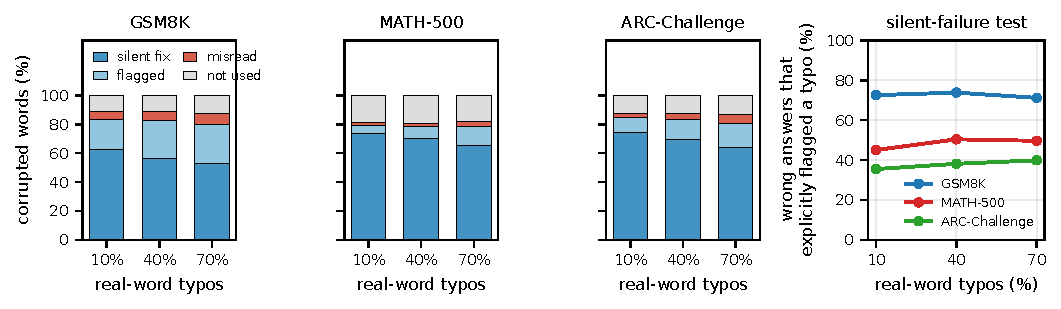
\includegraphics[width=0.96\textwidth]{fig3_repair.pdf}
\caption{Repair behaviour. Word-level alignment (first three panels) shows that
as the real-word share rises, silent fixing collapses and flagging and misreads
grow. The rightmost panel tests the pre-registered ``silent failure''
hypothesis: among \emph{wrong} answers, the fraction where the model explicitly
noticed a typo does not fall with the real-word share --- it is flat (GSM8K,
MATH-500) or rises (ARC). Real-word typos do not fail silently.}
\label{fig:repair}
\end{figure*}

Our proposal predicted that real-word typos would slip through unnoticed and
produce confident wrong answers, while non-word typos would trigger visible
self-correction. The first half is wrong.

Word-level alignment shows the expected shift in handling: on GSM8K, silent
correct fixing falls from $62.3\%$ of typos at $\rho{=}10$ to $52.9\%$ at
$\rho{=}70$, while explicit flagging rises $21.0\to26.8\%$ and misreads rise
$5.4\to7.7\%$; the same monotone pattern holds on MATH-500 ($73.3\to65.5\%$
silent) and ARC ($74.5\to63.6\%$). Misreading is strongly associated with
failure: misread rates are $1.2$--$2.0\times$ higher in wrong answers than in
correct ones.

But the ``silent'' part of the hypothesis fails. Among GSM8K questions the model
got \emph{wrong}, the fraction in which it explicitly noticed at least one typo
is $72.5\%$, $73.8\%$, $71.2\%$ at $\rho=10,40,70$ --- flat. On ARC it
\emph{rises} ($35.5\to39.9\%$), and on MATH-500 it is flat-to-rising
($45.0\to49.6\%$). Real-word corruptions are noticed at least as often as
non-word ones.

The LLM judge on ARC explains why they still hurt. As the real-word share grows,
the judge's labels shift away from \textsc{silent\_readthrough}
($68.9\to56.4\%$) toward \textsc{explicit\_notice\_nofix} ($3.1\to4.8\%$) and,
most sharply, \textsc{misread\_wrong\_word} ($2.9\to9.2\%$, a $3.2\times$
increase) --- and these labels carry very different accuracies:
\textsc{silent\_readthrough} $84.1\%$ ($n{=}2159$),
\textsc{explicit\_notice\_fix} $77.2\%$ ($n{=}926$),
\textsc{explicit\_notice\_nofix} $59.1\%$ ($n{=}127$),
\textsc{misread\_wrong\_word} $57.9\%$ ($n{=}202$).

The mechanism is therefore \emph{noticed-but-unrecoverable}, not silent. The
model can tell that \texttt{east} is out of place; what it cannot do is
recover that the intended word was \texttt{eats}, because \texttt{east} is a
legal word in a legal position and the evidence needed to invert the corruption
has been destroyed. Non-word typos leave the correction target visible;
real-word typos do not. Detection is not the bottleneck --- inversion is.

\subsection{The lexical signature of typo stress is hedging}
\label{sec:doubt}

\begin{figure*}[t]
\centering
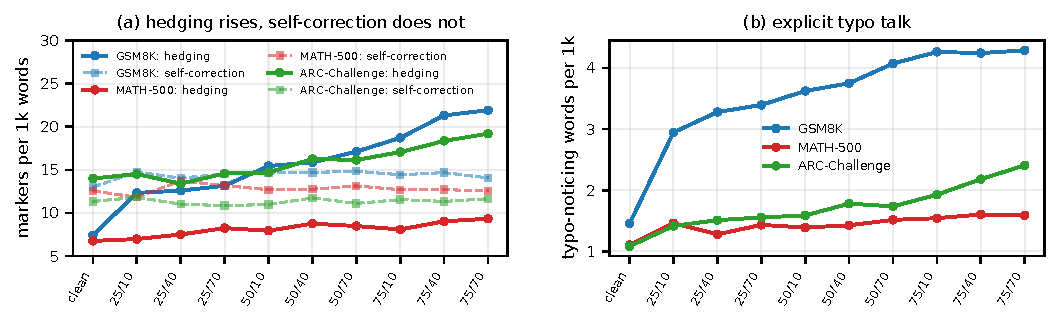
\includegraphics[width=0.78\textwidth]{fig4_doubt.pdf}
\caption{Self-doubt under typos. \textbf{Left}: total doubt markers per 1k
tokens. \textbf{Right}: the marker classes that move. Hedging
(``maybe'', ``perhaps'') grows sharply; classical self-correction
(``double-check'', ``let me recheck'', ``hold on'') is flat or declines.}
\label{fig:doubt}
\end{figure*}

Doubt-marker density rises with corruption on all three datasets: GSM8K
$20.4\to36.0$ per 1k tokens, ARC $24.7\to30.8$, MATH-500 $19.3\to21.9$. The
composition is the interesting part. On GSM8K the markers that grow are hedges
(\emph{maybe} $+5.66$/1k, \emph{wait} $+2.43$, \emph{or maybe/alternatively}
$+1.76$, \emph{perhaps} $+1.13$), while markers of deliberate verification
\emph{shrink} (\emph{double-check} $-0.35$, \emph{let me recheck} $-0.24$,
\emph{hold on} $-0.16$, \emph{wait, actually} $-0.09$). The ordering is
reproduced on MATH-500 and ARC. Typos do not make the model verify more; they
make it commit less --- a behavioural echo of \citet{huang2024}.

The LLM judge agrees with the lexical proxy: judged doubt and marker density
correlate at Pearson $r{=}0.53$ (Spearman $0.60$) on ARC and $r{=}0.85$
($0.92$) on GSM8K. Judged doubt rises with corruption on ARC ($2.49\to2.68$;
traces rated $\geq3$ go $56.8\to70.9\%$) and is higher for wrong than correct
answers in every configuration (ratio $1.06$--$1.14$). Expressed uncertainty is
a real but weak distress signal: it tracks failure without preventing it.

\subsection{Reasoning distillation does not confer robustness}
\label{sec:baseline}

\begin{table}[t]
\centering\small
\begin{tabular}{lcccc}
\toprule
 & \multicolumn{2}{c}{MATH-500} & \multicolumn{2}{c}{ARC-C} \\
\cmidrule(lr){2-3}\cmidrule(lr){4-5}
config & R1-7B & Qwen2.5 & R1-7B & Qwen2.5 \\
\midrule
clean          & 95.2 & 76.2 & 85.0 & 91.6 \\
typo25\_real10 & 93.9 & 75.5 & 86.5 & 92.2 \\
typo25\_real70 & 93.9 & 73.7 & 82.0 & 90.3 \\
typo50\_real10 & 92.8 & 72.8 & 81.9 & 90.6 \\
typo50\_real70 & 91.5 & 72.1 & 82.4 & 87.9 \\
typo75\_real10 & 89.1 & 68.0 & 80.7 & 87.4 \\
typo75\_real70 & 86.9 & 69.3 & 74.7 & 83.9 \\
\midrule
$\Delta$ clean$\to$75/70 & $-8.2$ & $-6.8$ & $-10.4$ & $-7.7$ \\
\bottomrule
\end{tabular}
\caption{Reasoning-distilled vs.\ non-reasoning model of the same family and
size, answered-only accuracy (\%), scored identically. The reasoning model is
far better on MATH-500 and far worse on ARC, but in both cases it loses
\emph{more} accuracy to typos than the instruct model.}
\label{tab:baseline}
\end{table}

Table~\ref{tab:baseline} compares R1-Distill-Qwen-7B with Qwen2.5-7B-Instruct,
same family, same size, scored by the identical pipeline. The absolute levels
differ enormously and in opposite directions --- the reasoning model is $19\pp$
better on MATH-500 and $6.6\pp$ worse on ARC --- but the \emph{slope} is what
matters, and on both datasets the reasoning model degrades more ($-8.2$ vs.\
$-6.8$ on MATH-500; $-10.4$ vs.\ $-7.7$ on ARC). Reasoning distillation buys
capability on clean text, not robustness to noisy text; if anything, the long
deliberation gives a misreading more opportunities to propagate.

\subsection{Every lightweight mitigation fails}
\label{sec:mitigations}

\begin{figure*}[t]
\centering
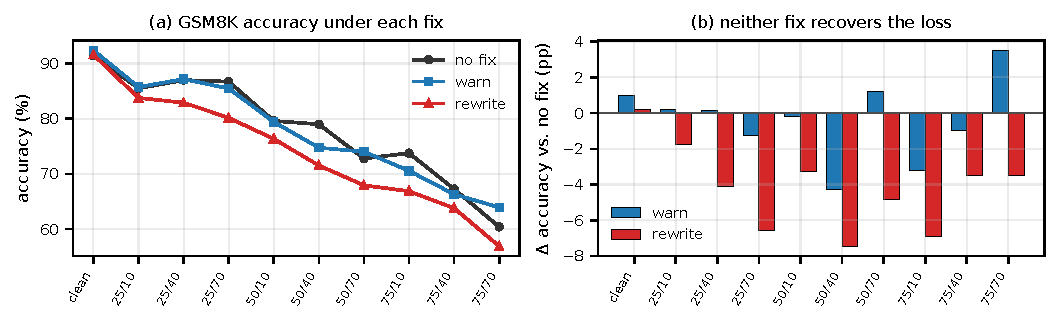
\includegraphics[width=0.7\textwidth]{fig5_fixes.pdf}
\caption{Prompt-level mitigations on GSM8K. Warning the model about typos is
null; asking it to rewrite the question before solving is actively harmful and
also shortens the reasoning trace by roughly a third.}
\label{fig:fixes}
\end{figure*}

We tested the three fixes proposed in our plan (Figure~\ref{fig:fixes}).

\paragraph{Warn.} Prepending \emph{``Note: the text may contain typos.''}
changes GSM8K accuracy by $-0.5\pp$ on average over the nine typo configurations
(range $-4.3$ to $+3.5$). Telling the model to be careful does not help, which
is exactly what \S\ref{sec:repair} predicts: it had already noticed.

\paragraph{Rewrite.} Instructing the model to \emph{``first rewrite the question
with all typos corrected, then solve it''} is worse than doing nothing in all
nine configurations, $-4.7\pp$ on average (up to $-7.5\pp$), and median
reasoning length drops from 1{,}214 to $\sim$730 tokens. The rewrite step
converts an open deliberation into a commitment: the model produces one
reconstructed question and solves \emph{that}, so any reconstruction error
becomes unrecoverable, and the budget spent reconstructing is taken from the
budget spent reasoning.

\paragraph{Spell check.} An external spell checker (\texttt{pyspellchecker},
edit distance $\leq2$, skipping protected spans, short words and acronyms) run
before the model sees the text restores the original word for $40.2\%$ of all
$68{,}739$ GSM8K typos --- but the breakdown by real-word share is decisive:
$54.9\%$ at $\rho{=}10$, $39.9\%$ at $\rho{=}40$ and $25.8\%$ at $\rho{=}70$
(22{,}913 typo words each).

A spell checker therefore recovers over half of the corruptions when only 10\%
are real words and barely a quarter when 70\% are --- an upper bound on what any
dictionary-based front-end can do, because a real-word typo is by construction
invisible to a dictionary. It also introduces its own errors, changing a further
$8{,}157$ words to something other than the original. The mitigation is
structurally blind to exactly the corruption class that \S\ref{sec:realword}
identifies as most damaging.

%-------------------------------------------------------------------------------
\section{Discussion}
\label{sec:discussion}

Three things follow from these results.

\textbf{Benchmark scores overstate real-world accuracy.} A 7B reasoning model
reported at $91\%$ on GSM8K delivers $60\%$ once three-quarters of the content
words carry a human-plausible typo, and $86\%$ at a mild and entirely realistic
$25\%$ rate --- none of which is visible in a score computed on copy-edited text.

\textbf{The dangerous corruption is the one that looks fine.} Our per-typo
analysis, our controlled paired test and our spell-checker measurement all point
the same way: the real-word channel dominates. This reframes the tokenization
account of \citet{chai2024}. Tokenizer fragmentation is real, but it is also
\emph{self-announcing} --- a fragmented word is visibly odd, and
\S\ref{sec:repair} shows the model repairs those silently and successfully most
of the time. The real-word channel produces no such signal, and no
dictionary-based defence can see it.

\textbf{Noticing is not repairing.} We set out to find silent failures and found
loud ones. The model flags the corruption, hedges about it, thinks $64\%$
longer, and still answers wrong, while the vocabulary of verification
(``double-check'', ``let me recheck'') declines under stress. This is the
input-side analogue of \citet{huang2024}, and it explains why interventions
aimed at \emph{detection} do nothing or backfire. A mitigation that could work
would have to preserve ambiguity rather than resolve it --- carrying several
candidate readings of a suspicious word through the reasoning --- instead of
forcing a single reconstruction up front, which is what our \emph{rewrite}
condition does and why it loses $4.7\pp$.

%-------------------------------------------------------------------------------
\section{Limitations}
\label{sec:limitations}

\textbf{One model, one sample.} All headline results come from a single 7B
reasoning model at one decoding setting with $n{=}1$ sample per question. Our
plan called for several samples; the API budget did not permit it, so we cannot
separate typo effects from decoding variance at the level of an individual
question. The aggregate effects are far larger than plausible sampling noise
(McNemar $p<10^{-6}$ on $n{=}480$ paired items), but generalisation to larger
reasoning models is untested. We also planned GPQA-Diamond and ran
ARC-Challenge instead after the GPQA grid could not be completed in time; ARC is
easier and its four options provide answer-side redundancy, so our
multiple-choice results likely \emph{understate} the tax on harder science
questions.

\textbf{Measurement caveats.} The ARC \texttt{clean} condition answered
455/500 questions versus 461--489 for the typo conditions, so the clean-vs-typo
gap on ARC is, if anything, understated; the paired flip analysis
(Table~\ref{tab:fullflips}) is immune to this. Real-word detection uses the
NLTK English lexicon, which contains rare words a reader would not recognise,
making our real-word ratio a slight over-count.

\textbf{Mitigations and human validation.} The three fixes were evaluated on
GSM8K only, and the spell-check arm was served with a different generation cap
(4{,}096 tokens), giving it a lower clean baseline (83.7\%); its restoration
statistics are unaffected, but its accuracy numbers are only interpretable
within that run. We also did not run the
planned human study confirming that corrupted questions remain answerable by
people, so part of the tax at $r{=}75$ may be irreducible ambiguity; the
$r{=}25$ and $r{=}50$ conditions, where the effects are already large and
significant, are much less exposed to this concern.

%-------------------------------------------------------------------------------
\section{AI Disclosure and Reflection}
\label{sec:ai}

\paragraph{What we used AI for.} We used GitHub Copilot with Claude as a coding
assistant throughout: scaffolding the typo generator and the inference runner,
writing the ten analysis scripts, generating the matplotlib figure code, and
drafting and copy-editing sections of this paper.
\texttt{Llama-3.3-70B-Instruct} is an experimental component (the judge of
\S\ref{sec:setup}), not a writing tool. All design decisions --- the two-axis
grid, the technique weights, the strict answer-extraction policy, the paired
McNemar design, the judge rubric --- were ours, and every number here was
produced by our scripts from the raw generation logs.

\paragraph{What went wrong.} Two failures are worth recording. AI-written
analysis code produced a plausible-looking spell-checker recovery table whose
values were all exact multiples of 500; the underlying per-row metadata turned
out to be constant across a whole file, and we recomputed the statistic from the
raw edit records. Separately, an AI-generated supplementary table disagreed with
our main tables by 1--2 points because it used a laxer answer extractor; we
regenerated it with the strict scorer. Both errors survive a read-through and
only fail a consistency check.

\paragraph{Reflection.} The assistant was most valuable for mechanical breadth
--- ten analyses sharing one loading and scoring path, consistent figure code
--- and least trustworthy exactly where it looked most competent: producing
well-formatted tables of numbers. Our working rule became that no number enters
the paper unless it can be re-derived from the raw JSONL by a script we have
read line by line. The main scientific lesson was to distrust
agreement-with-expectation: the ``silent failure'' result we expected would have
been easy to write up, and it took the judge's own accuracy-by-label breakdown
to show us the mechanism was the opposite.

%-------------------------------------------------------------------------------
\section{Conclusion}

Typos impose a large and systematic tax on reasoning LLMs: up to $31\pp$ on
GSM8K, monotone in corruption rate, and concentrated in corruptions that produce
other valid English words. The failure mode is not silence but
noticed-but-unrepairable misreading, the trace signature is hedging rather than
verification, reasoning distillation does not protect against it, and none of
the obvious prompt-level or dictionary-level fixes work. Robustness to the text
people actually type will have to be built deliberately. All code is in the
project repository and the raw generation logs are on the Hugging Face Hub
(\texttt{ronshtricker/typo-reasoning-results}); every result here is regenerated
by \texttt{download\_data.py} followed by \texttt{run\_all.py}.

\bibliography{custom}

\clearpage
\onecolumn
%-------------------------------------------------------------------------------
\appendix

\section{Full accuracy grid}
\label{app:acc}
\begin{table}[!ht]
\centering\small
\begin{tabular}{l rrr rrr rrr}
\toprule
 & \multicolumn{3}{c}{GSM8K} & \multicolumn{3}{c}{MATH-500} & \multicolumn{3}{c}{ARC-Challenge} \\
\cmidrule(lr){2-4}\cmidrule(lr){5-7}\cmidrule(lr){8-10}
config & acc & $n_a$ & tok & acc & $n_a$ & tok & acc & $n_a$ & tok \\
\midrule
clean & 91.4 & 500 & 1582 & 95.2 & 496 & 2927 & 84.7 & 485 & 1172 \\
typo25\_real10 & 85.5 & 497 & 1912 & 93.9 & 495 & 2945 & 86.5 & 487 & 1222 \\
typo25\_real40 & 87.0 & 500 & 1814 & 93.4 & 498 & 3111 & 85.6 & 486 & 1246 \\
typo25\_real70 & 86.7 & 497 & 1843 & 93.9 & 494 & 2992 & 82.0 & 489 & 1234 \\
typo50\_real10 & 79.6 & 500 & 2024 & 92.8 & 498 & 2939 & 81.9 & 487 & 1298 \\
typo50\_real40 & 79.0 & 500 & 2084 & 91.4 & 498 & 3085 & 82.5 & 485 & 1357 \\
typo50\_real70 & 72.8 & 500 & 2094 & 91.5 & 496 & 3087 & 82.4 & 484 & 1329 \\
typo75\_real10 & 73.8 & 488 & 2084 & 89.1 & 494 & 2945 & 80.7 & 488 & 1381 \\
typo75\_real40 & 67.3 & 495 & 2594 & 88.1 & 496 & 3125 & 77.3 & 485 & 1413 \\
typo75\_real70 & 60.4 & 480 & 2306 & 86.9 & 497 & 3138 & 74.7 & 486 & 1453 \\
\bottomrule
\end{tabular}

\caption{Answered-only accuracy (\%), number of answered questions ($n_a$), and
mean generated tokens, for all configurations and datasets.}
\label{tab:fullacc}
\end{table}

\section{Paired flips and significance}
\label{app:flips}
\begin{table}[!ht]
\centering\small
\begin{tabular}{l rrr rrr rrr}
\toprule
 & \multicolumn{3}{c}{GSM8K} & \multicolumn{3}{c}{MATH-500} & \multicolumn{3}{c}{ARC-Challenge} \\
\cmidrule(lr){2-4}\cmidrule(lr){5-7}\cmidrule(lr){8-10}
config & r$\to$w & w$\to$r & $p$ & r$\to$w & w$\to$r & $p$ & r$\to$w & w$\to$r & $p$ \\
\midrule
typo25\_real10 & 48 & 19 & 6.2e-04 & 12 & 7 & 0.359 & 21 & 27 & 0.470 \\
typo25\_real40 & 40 & 18 & 0.006 & 15 & 9 & 0.307 & 25 & 31 & 0.504 \\
typo25\_real70 & 43 & 19 & 0.003 & 15 & 9 & 0.307 & 39 & 25 & 0.104 \\
typo50\_real10 & 78 & 19 & $<$1e-6 & 18 & 9 & 0.124 & 38 & 26 & 0.169 \\
typo50\_real40 & 83 & 21 & $<$1e-6 & 22 & 6 & 0.005 & 37 & 25 & 0.162 \\
typo50\_real70 & 108 & 15 & $<$1e-6 & 25 & 9 & 0.010 & 42 & 27 & 0.092 \\
typo75\_real10 & 102 & 14 & $<$1e-6 & 34 & 5 & 7.3e-06 & 52 & 32 & 0.038 \\
typo75\_real40 & 136 & 17 & $<$1e-6 & 39 & 7 & 4.9e-06 & 59 & 26 & 5.2e-04 \\
typo75\_real70 & 164 & 14 & $<$1e-6 & 46 & 7 & $<$1e-6 & 73 & 23 & $<$1e-6 \\
\bottomrule
\end{tabular}

\caption{Right-to-wrong and wrong-to-right flips against the \texttt{clean}
condition on jointly answered questions, with continuity-corrected McNemar
$p$-values.}
\label{tab:fullflips}
\end{table}

\section{Self-doubt markers}
\label{app:doubt}
\begin{table}[!ht]
\centering\small
\begin{tabular}{l rr rr rr}
\toprule
 & \multicolumn{2}{c}{GSM8K} & \multicolumn{2}{c}{MATH-500} & \multicolumn{2}{c}{ARC-Challenge} \\
\cmidrule(lr){2-3}\cmidrule(lr){4-5}\cmidrule(lr){6-7}
config & s.corr. & hedge & s.corr. & hedge & s.corr. & hedge \\
\midrule
clean & 13.0 & 7.4 & 12.6 & 6.8 & 11.1 & 13.6 \\
typo25\_real10 & 14.7 & 12.3 & 11.8 & 7.0 & 11.8 & 14.5 \\
typo25\_real40 & 14.0 & 12.6 & 13.7 & 7.5 & 11.0 & 13.4 \\
typo25\_real70 & 14.5 & 13.2 & 13.2 & 8.2 & 10.8 & 14.6 \\
typo50\_real10 & 14.6 & 15.4 & 12.7 & 7.9 & 11.0 & 14.7 \\
typo50\_real40 & 14.7 & 15.9 & 12.7 & 8.8 & 11.6 & 15.9 \\
typo50\_real70 & 14.8 & 17.1 & 13.1 & 8.5 & 11.1 & 16.1 \\
typo75\_real10 & 14.4 & 18.7 & 12.7 & 8.1 & 11.5 & 17.1 \\
typo75\_real40 & 14.7 & 21.3 & 12.7 & 9.0 & 11.3 & 18.4 \\
typo75\_real70 & 14.1 & 21.9 & 12.5 & 9.3 & 11.6 & 19.2 \\
\bottomrule
\end{tabular}

\caption{Doubt-marker density per 1k generated tokens, per configuration.}
\label{tab:fulldoubt}
\end{table}

\section{Word-level repair behaviour}
\label{app:repair}
\begin{table}[!ht]
\centering\small
\begin{tabular}{l r rrrr}
\toprule
dataset / config & \#words & silent fix & flagged & misread & not used \\
\midrule
\multicolumn{6}{l}{\emph{GSM8K}} \\
\quad typo25\_real10 & 3656 & 73.2 & 11.9 & 2.9 & 11.9 \\
\quad typo25\_real40 & 3673 & 70.2 & 15.1 & 4.3 & 10.4 \\
\quad typo25\_real70 & 3650 & 64.6 & 19.3 & 4.8 & 11.3 \\
\quad typo50\_real10 & 7202 & 65.8 & 18.7 & 4.7 & 10.9 \\
\quad typo50\_real40 & 7179 & 60.6 & 23.4 & 5.2 & 10.8 \\
\quad typo50\_real70 & 7173 & 55.9 & 25.3 & 6.6 & 12.2 \\
\quad typo75\_real10 & 9833 & 55.8 & 26.1 & 6.9 & 11.3 \\
\quad typo75\_real40 & 9945 & 47.4 & 32.9 & 8.3 & 11.4 \\
\quad typo75\_real70 & 9528 & 46.2 & 30.9 & 9.6 & 13.3 \\
\multicolumn{6}{l}{\emph{MATH-500}} \\
\quad typo25\_real10 & 1882 & 78.0 & 2.3 & 1.2 & 18.4 \\
\quad typo25\_real40 & 1901 & 73.1 & 5.8 & 1.6 & 19.5 \\
\quad typo25\_real70 & 1881 & 71.4 & 10.2 & 1.7 & 16.8 \\
\quad typo50\_real10 & 3661 & 75.0 & 4.3 & 1.4 & 19.4 \\
\quad typo50\_real40 & 3661 & 70.2 & 8.3 & 2.3 & 19.2 \\
\quad typo50\_real70 & 3651 & 67.2 & 11.3 & 2.9 & 18.6 \\
\quad typo75\_real10 & 5282 & 70.4 & 8.2 & 2.1 & 19.3 \\
\quad typo75\_real40 & 5260 & 68.4 & 9.6 & 2.4 & 19.5 \\
\quad typo75\_real70 & 5297 & 62.2 & 15.2 & 4.0 & 18.5 \\
\multicolumn{6}{l}{\emph{ARC-Challenge}} \\
\quad typo25\_real10 & 1964 & 80.0 & 5.8 & 2.1 & 12.1 \\
\quad typo25\_real40 & 1981 & 74.8 & 9.1 & 3.1 & 13.1 \\
\quad typo25\_real70 & 1988 & 69.6 & 12.2 & 5.3 & 12.9 \\
\quad typo50\_real10 & 3932 & 76.9 & 8.1 & 2.5 & 12.5 \\
\quad typo50\_real40 & 3747 & 71.8 & 11.7 & 3.6 & 12.9 \\
\quad typo50\_real70 & 3887 & 66.7 & 14.2 & 5.3 & 13.7 \\
\quad typo75\_real10 & 5847 & 71.0 & 13.4 & 3.4 & 12.2 \\
\quad typo75\_real40 & 5777 & 65.8 & 16.3 & 5.0 & 12.8 \\
\quad typo75\_real70 & 5769 & 59.4 & 20.3 & 6.9 & 13.3 \\
\bottomrule
\end{tabular}

\caption{Word-level classification of every corrupted word: silently fixed,
explicitly flagged, misread, or not used in the trace.}
\label{tab:fullrepair}
\end{table}

\end{document}
